\documentclass{zkdl-template-105x135-nohead}

\usepackage{opencolor}

\title{\huge\sffamily\bfseries ZKDL Lecture Notes}
\author{\Large\sffamily by \emph{Distributed Lab}}
\date{\sffamily \monthname[\the\month] \ \the\year \\ \vspace{1mm} Version 0.1}

\begin{document}

    \pagestyle{fancy}

% --- Drawing a book cover ---

    \colorlet{coverBackground}{oc-gray-0}
    \colorlet{coverBoxBackground}{oc-gray-7}

    \pagecolor{coverBackground}
    \begin{tcolorbox}[
        standard jigsaw,
        colframe=coverBoxBackground,
        colback=oc-gray-3,
        width=\textwidth,
        halign=center,
        valign=center,
    %opacityback=0,
        arc=1em,
        shadow={4mm}{-3mm}{0mm}{black!30!white},
        enhanced,
        boxrule=5pt,
        rightrule=9pt,
        bottomrule=9pt]
        \maketitle
    \end{tcolorbox}

% Include figure below

    \vspace{1.5cm}
    \begin{figure}[h]
        \centering
        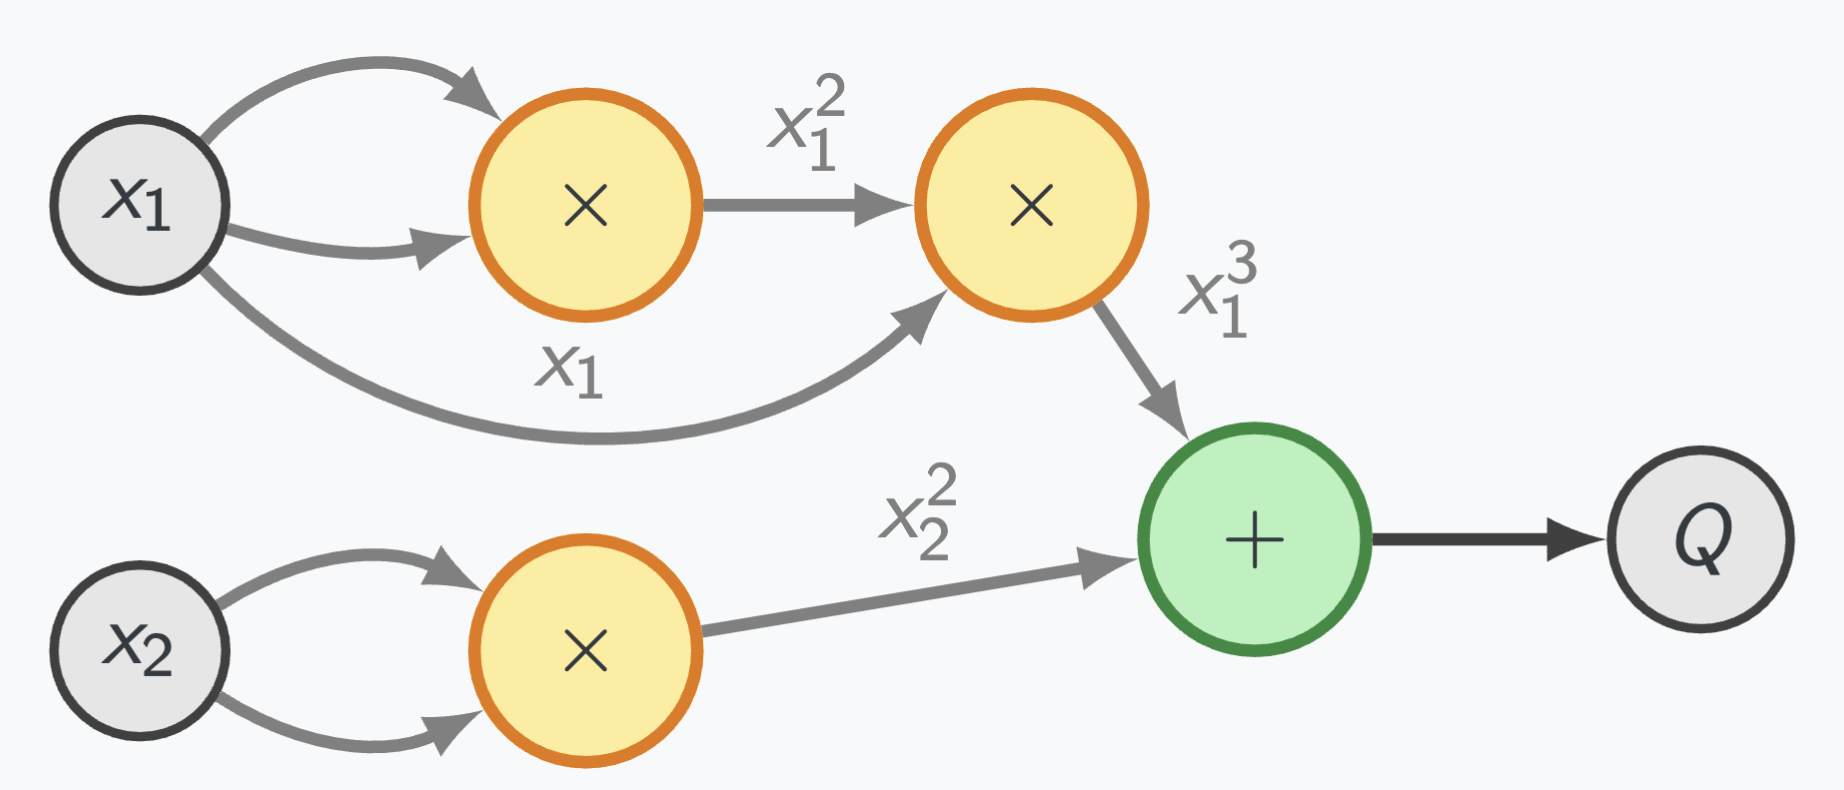
\includegraphics[width=0.8\textwidth]{lectures/images/cover-image-1.png}
    \end{figure}

    \thispagestyle{empty}
    \pagebreak

%  Inverse title page

    \thispagestyle{empty}
    \pagebreak
    
    \pagecolor{white}
    
    \begin{abstract}
        \fontsize{7}{8}\selectfont
        Due to the rise of zero-knowledge technologies and their applications in
        various fields such as Blockchain or anonymous identity management, it is
        essential to develop a comprehensive understanding of the underlying
        mechanisms. However, the existing resources on the topic are either too
        high-level or too low-level, making it hard for regular practicing engineers
        to understand the practical implications of zero-knowledge protocols.
    
        This book aims to bridge this gap by providing a complete, practical guide
        to the state-of-the-art techniques in zero-knowledge cryptography, such as
        $\Sigma$-protocols, zk-SNARKs (Groth16 in particular), PlonK and more. We
        gathered all the necessary information in one place, and tried to make it
        easy to follow, with numerous examples and code snippets. We attach
        exercises to each chapter to help you understand the material better.
        Despite the book's practical focus, we preserve the mathematical rigor where
        suitable and necessary.
    \end{abstract}
    
    \newpage
% --- Table of Contents ---

    \pagecolor{white}

    \tableofcontents

    \pagebreak

% --- Content ---

    \section*{Preface}

    \subfile{preface}

    \section{Group Theory and Polynomials} \label{section:math-crypto-1}

    \subfile{lectures-105-135/1-math}

    \section{Basics of Security Analysis}\label{section:math-crypto-2}

    \subfile{lectures-105-135/2-math-and-crypto}

    \section{Field Extensions and Elliptic Curves}

    \subfile{lectures-105-135/3-ec}\label{section:field_extensions}

    \section{Projective Coordinates and Pairing}

    \subfile{lectures-105-135/4-pairing}

    \section{Commitment Schemes} \label{section:commitments}

    \subfile{lectures-105-135/5-commitments} 

    \section{Introduction to Zero-Knowledge Proofs} \label{section:intro-zk}

    \subfile{lectures-105-135/6-intro-zk}

    \section{Sigma Protocols} \label{section:sigma}

    \subfile{lectures-105-135/7-sigma}

    \section[Arithmetic Circuits. R1CS]{Introduction to SNARKs. Arithmetic Circuits. R1CS} \label{section:r1cs}

    \subfile{lectures-105-135/8-circuits}\label{secation:circuits}

    \section[Quadratic Arithmetic Program]{Quadratic Arithmetic Program. Probabilistically Checkable Proofs} \label{section:qap}

    \subfile{lectures-105-135/9-qap-pcp}

    \section[Pairing-based SNARKs]{Pairing-based SNARKs. Pinocchio and Groth16} \label{section:groth16}

    \subfile{lectures-105-135/10-groth}

    \section{Circom} \label{section:circom}

    \subfile{lectures-105-135/11-circom} 

    \section{PlonK} \label{section:plonk}

    \subfile{lectures-105-135/12-plonk}

    % Contacy page

    \newpage
    \pagestyle{empty}
    
    \ifodd\value{page}
        \newpage
    \fi
    
    \vspace*{\fill}
    
    \begin{center}
        contact@distributedlab.com
    \end{center}
    
    \vspace*{\fill}

\end{document}
